\section{Prompt sensitivity}
\label{app:prompt-sensitivity}

Paraphrasing the decode prompt changes the wording but rarely the content (\tabref{psens}).
For PACS cluster labels and two-paper midpoint descriptions, we decoded each point under eight semantically equivalent prompts, with generation settings held fixed.
We score the eight outputs of a point by SBERT cosine.
Two different PACS nodes decoded under one prompt have mean cosine $.463$, and two different midpoints have mean cosine $.244$.

The eight PACS-label prompts follow (1 is the wording of \secref{cluster-labeling}).
\begin{enumerate}[leftmargin=1.8em,itemsep=2pt,parsep=0pt,topsep=4pt]
\footnotesize
\item In 2 to 3 words, name the scientific field that all of these documents belong to. Reply with only the field name.
\item Using 2 or 3 words, state the scientific field shared by all of these documents. Answer with the field name only.
\item What scientific field do all of these documents belong to? Answer in 2-3 words, nothing else.
\item Name, in at most three words, the research field common to these documents. Output only the name.
\item Give the shared scientific field of these documents as a 2-3 word phrase and nothing more.
\item Identify the field of science that covers all of these documents. Reply with a two or three word field name only.
\item In a phrase of two to three words, what is the common scientific field of these documents? Reply with the phrase alone.
\item Summarise the scientific field of these documents in 2-3 words. Do not add any explanation.
\end{enumerate}

The eight midpoint-description prompts follow (1 is the $2$--$3$ sentence combined-idea prompt).
\begin{enumerate}[leftmargin=1.8em,itemsep=2pt,parsep=0pt,topsep=4pt]
\footnotesize
\item You have read two research papers and hold a single combined idea. In 2 to 3 sentences, describe the combined research idea. Reply with the description only.
\item Describe, in two or three sentences, the single research idea that combines the two papers you have read. Output only the description.
\item What research idea sits between the two papers you have read? Answer in 2-3 sentences.
\item In at most three sentences, state the merged research idea formed from the two papers.
\item Summarise the blended research idea of the two internalised papers in two to three sentences.
\item Give a 2-3 sentence description of the research idea that fuses the two papers you hold.
\item Express, in two or three sentences, the combination of the two papers as one research idea.
\item Write two or three sentences describing the single idea that unites the two papers you read.
\end{enumerate}

PACS labels mostly stay the same string.
Eight prompts produce $3.2$ distinct labels on average.
The most frequent label appears in $72\%$ of the outputs, and $51\%$ of prompt pairs match exactly.

Midpoint descriptions produce a new string under every prompt.
Mean pairwise cosine is $.705$.
The lowest pair is $.507$, still well above the $.244$ baseline between different points.
Two descriptions of the same midpoint therefore remain closer than descriptions of two different midpoints, even when the prompt changes.

The wording in the paper is typical of this paraphrase set.
Similarity to that wording equals or exceeds the mean pairwise similarity ($.841$ for labels, $.705$ for midpoints).

\begin{table}[h]
\centering
% Six columns with two long headers ran ~43pt past \textwidth at \footnotesize.
% One size step plus tighter column padding brings it inside the margin.
\scriptsize
\setlength{\tabcolsep}{4pt}
\caption{Prompt sensitivity. $K$ is the number of semantically equivalent prompts per point, the first being the one the paper reports. \emph{mean pairwise sim.}\ averages SBERT cosine over prompt pairs for the same point; \emph{sim.\ to the reported prompt} compares the other seven against it. \emph{identical strings} is the fraction of those prompt pairs that emit the same text after lowercasing. Two different PACS nodes decoded under one prompt have mean cosine $.463$. Two different midpoints decoded under one prompt have mean cosine $.244$.}
\label{tab:psens}
% auto-generated by workflow/scripts/groupc/psens_score.py (issue #73) -- do not edit
\begin{tabular}{lrrrrr}
\toprule
decode family & units & $K$ & mean pairwise sim. & sim.\ to the reported prompt & identical strings \\
\midrule
PACS node labels (2--3 words) & 30 & 8 & 0.787 & 0.841 & 51\% \\
% single-paper descriptions row (40 units, .888 / .884 / 0%, null .162) omitted: that family is not reported in the paper.
two-paper midpoint descriptions & 40 & 8 & 0.705 & 0.705 & 0\% \\
\bottomrule
\end{tabular}

\end{table}


\begin{figure}[t]
\centering
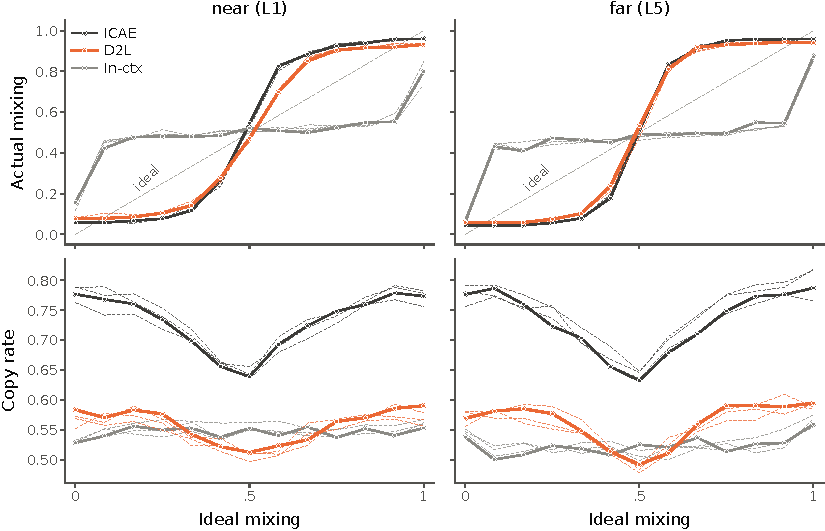
\includegraphics[width=\linewidth]{../../figs/psens_edge_curves.pdf}
\caption{Decoded abstracts along the A--B interpolation under paraphrase, near pairs (left) and far pairs (right). Solid lines are the wording reported in \secref{fusion} and dashed lines its three paraphrases. \emph{Top}, where the decoded abstract lands on the A$\to$B axis in SBERT space against the requested mix weight, with the diagonal marking proportional tracking. \doctolora and \texttt{ICAE} sit near a source paper at the endpoints and blend through the middle, while in-context prompting stays near the midpoint across the whole interior. \emph{Bottom}, verbatim copy rate. \texttt{ICAE} sits above the other two everywhere, and \doctolora and in-context prompting overlap. Paraphrase moves every curve by less than the gap between methods.}
\label{fig:psens-edge}
\end{figure}

We paraphrased the four-to-six sentence abstract prompt from \secref{fusion} three times. The wordings are listed as follows:
\begin{enumerate}[leftmargin=1.8em,itemsep=2pt,parsep=0pt,topsep=4pt]
\footnotesize
\item Write a detailed abstract (four to six sentences) describing this research topic: its problem, methods, and findings.
\item In four to six sentences, write a detailed abstract for this research topic, covering the problem it addresses, the methods it uses, and its findings.
\item Produce a detailed abstract of this research topic -- its problem, its methods and its findings -- in four to six sentences.
\item Describe this research topic as a detailed abstract of four to six sentences, stating the problem addressed, the methods used and the results obtained.
\end{enumerate}
For each wording, we decoded 20 near pairs and 20 far pairs at 13 mix weights for each method (\doctolora, in-context prompting, \texttt{ICAE}), totaling 6240 decodes. The in-context baseline used the same two-document template from Appendix~\ref{app:edge-protocol}, changing only the instruction.

Decoded abstracts closely tracked the requested mix for every wording (see \figref{psens-edge}). 
For \doctolora, slope of decoded position versus mix weight ranged from 1.11 to 1.20.
For \texttt{ICAE}, 1.19 to 1.24. In-context prompting ranged from 0.29 to 0.41. No wording changed the slope by more than 0.04.
Copy rate stayed consistent. \texttt{ICAE} copied the most, averaging 0.72 to 0.75, and never matched the other methods. 
\doctolora and in-context prompting were both near 0.55.

Changing the mix point rewrote abstracts much more than changing the prompt. Abstracts at the same point under different wordings had SBERT cosine similarity of 0.886 for \doctolora, 0.924 for in-context prompting, and 0.923 for \texttt{ICAE}. Abstracts at different points under one prompt had much lower cosine (0.146 for \doctolora, 0.256 for in-context prompting, 0.125 for \texttt{ICAE}).
